\section{Exploring the incidents' temporal distribution}

\subsection*{Question 5.1}
\textit{How do the different types of incidents (as represented by Event Clearance Group) vary in number over the different years? Do you see different types of incidents having the same temporal variation pattern over the same year(s)?}


\subsection*{Question 5.2}
\textit{How do the different types of reported incidents (as represented by Initial Type Group) vary over the 24 hours of a day, for the entire data collection? Are there certain hours having a higher rate of reported incidents?}


\subsection*{Question 5.3}
\textit{How long does it take to clear incidents, as a function of the hour when they were reported? For example, do incidents reported at noon get cleared faster than incidents reported in the middle of the night?}

The visualization uses a bar chart.
The x-axis represents the hour of the day, while the y-axis shows the average resolution time for incidents reported in the given hour.
Color overloads the value showed in the y-axis.
The average line helps to compare particular time slots with the average behaviour.

Best practices for visualization suggests to use line charts instead of bar charts for continuous values like time.
In this case, however, we have discretized time into buckets of one hour and aggregated them together to compute the average.
In other words, we treat time as a discrete ordinal value.

\begin{figure}[h]
	\centering
	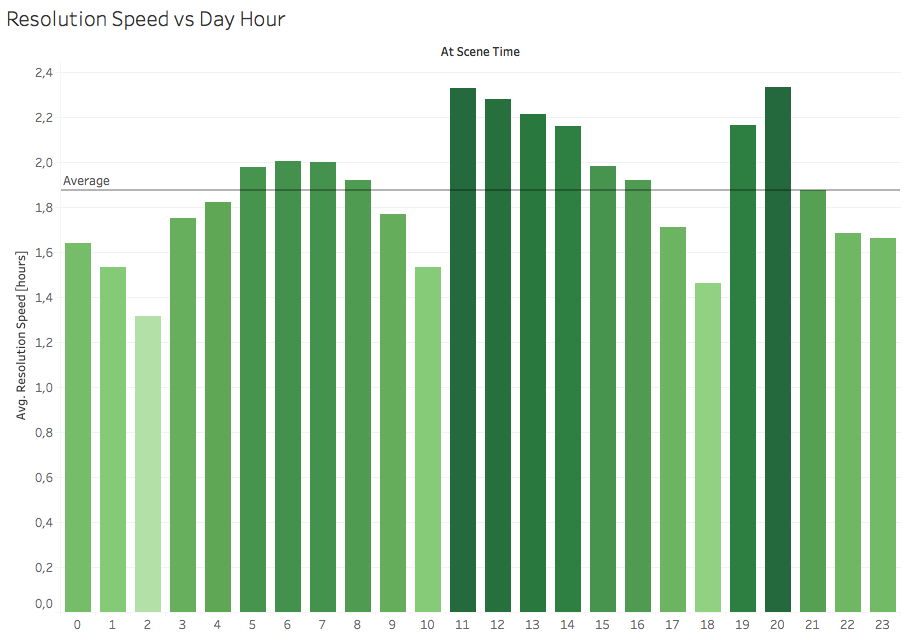
\includegraphics[width=0.9\columnwidth]{figures/5_3_resolution_speed_vs_hour}
	\caption{Resolution speed of incidents reported in different hour. The sheet is called \textit{Resolution Speed vs Day Hour} in Tableau.}
	\label{fig:5_3_resolution_speed_vs_hour}
\end{figure}

\cref{fig:5_3_resolution_speed_vs_hour} shows the visualization.
We can notice that:
\begin{itemize}
    \item The average time required to close incidents is not constant over the different hours of the day.
    \item Incidents that happens in the slots $11 - 14$ and $19 - 20$ take significant longer to be closed.
    \item Incidents that happens in the early morning ($5 - 7$) require on average more time than the incidents in the night and late morning ($9 - 10$).
    \item The time slots between $5 - 7$, $11 - 14$ and $19 - 20$ have a faster resolution speed.
\end{itemize}

To sum up, there is a correlation between the hour of the day and the time required to close incidents.
The visualization fully answers the question.

We have created a second visualization to check if this behaviour is common to all years.
The visualization uses again bar charts, one for each year.
The last column shows the average over all years as a reference for comparisons.
The axises are swapped in comparison to \cref{fig:5_3_resolution_speed_vs_hour} to better fit the screen.

\begin{figure}[h]
	\centering
	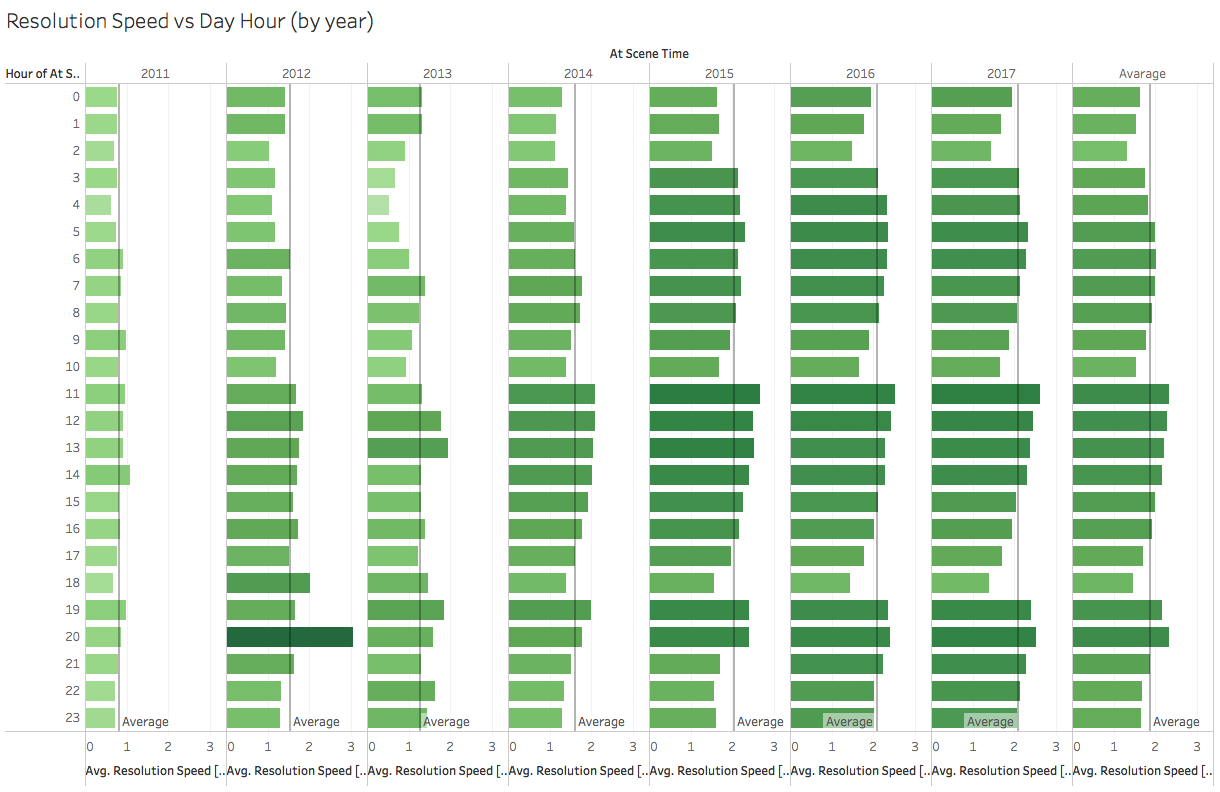
\includegraphics[width=0.9\columnwidth]{figures/5_3_resolution_speed_vs_hour_by_year}
	\caption{Resolution speed of incidents reported in different hour by year. The sheet is called \textit{Resolution Speed vs Day Hour (by year)} in Tableau.}
	\label{fig:5_3_resolution_speed_vs_hour_by_year}
\end{figure}

From \cref{fig:5_3_resolution_speed_vs_hour_by_year} we can notice that:
\begin{itemize}
    \item In $2011$ incidents are closed much faster than the average. There are some hours with a slightly higher resolution speed ($9$, $14$, $19$), but the difference with the rest of the day is small.
    \item Incidents that happens at $20$ in year $2012$ seems to take much longer to close than the average. This is probably due to the outliers discussed in \cref{sec:question3}, since both have very long resolution times and are in that slot of time.
    \item Years $2013$ have some picks in the slots $12 - 13$ and $18 - 20$. However, there are probably missing data for this year (see \cref{sec:question1}, so the confidence for this observation is low.
    \item Years $2014$, $2015$, $2016$ and $2017$ have a behaviour identical to the average over all years.    
\end{itemize}

To sum up, the resolution speed for the different hours of the day seems to be stable over years $2014$ to $2017$.
The previous years have slightly different behaviour, but still share some patterns.
Incidents that occurs in slots $5 - 7$, $11 - 14$ and $19 - 20$ take more time to be closed, while incidents between this slots are closed much faster.
